\documentclass[11pt,a4paper, uplatex]{jsarticle}
%
\usepackage{amsmath,amssymb}
\usepackage{bm}
\usepackage[dvipdfmx]{graphicx}
\usepackage{ascmac}
\usepackage{listings,jlisting}
\usepackage{underscore}
\usepackage{subfig}
\lstset{
    frame=single,
    numbers=left,
    tabsize=2
}
%
\setlength{\textwidth}{\fullwidth}
\setlength{\textheight}{40\baselineskip}
\addtolength{\textheight}{\topskip}
\setlength{\voffset}{-0.2in}
\setlength{\topmargin}{0pt}
\setlength{\headheight}{0pt}
\setlength{\headsep}{0pt}
%
\newcommand{\divergence}{\mathrm{div}\,}  %ダイバージェンス
\newcommand{\grad}{\mathrm{grad}\,}  %グラディエント
\newcommand{\rot}{\mathrm{rot}\,}  %ローテーション
%
\title{メディア情報学実験・音声認識 第一週課題レポート}
\author{1510151  栁 裕太}
\date{\today}
\begin{document}

\maketitle
\section{プログラム穴埋め}

\subsection{ad2fb.c}

\begin{lstlisting}[language=c, caption=\texttt{ad2fb}関数一部]
  for(j=0; j<NUMCHANS; j++) {
  m[i_frame][j] = 0;
  Aj = 0;
  for(k=klo[j]; k<kc[j]; k++) {
    /* ここから穴埋めしたエリア */
    W_kj = ((double)(k) - klo[j]) / (kc[j] - klo[j]);
    m[i_frame][j] += W_kj * pow(X[k], 2);
    Aj += W_kj;
    /* 穴埋めしたエリアおわり */
  }
  for(k=kc[j]; k<=khi[j]; k++) {
    /* ここから穴埋めしたエリア */
    W_kj = ((double)(khi[j]) - k) / (khi[j] - kc[j]);
    m[i_frame][j] += W_kj * pow(X[k], 2);
    Aj += W_kj;
    /* 穴埋めしたエリアおわり */
  }
  /* フィルタの面積が等しくなるように正規化 */
  m[i_frame][j] /= Aj;
\end{lstlisting}

\subsection{fb2mfcc.c}

\begin{lstlisting}[language=c, breaklines = true, caption=\texttt{fb2mfcc}関数一部]
  void fb2mfcc(int n_frame, /* フレーム数                 */
               float **m,   /* フィルタバンク              */
               float **c,   /* MFCC (フレーム x 次元)     */
               int P,       /* フィルタバンクのチャネル数     */
               int Q)       /* MFCCの次元                */
  {
    int i_frame;
    int i, j;
    double mfnorm, pi_factor, x, sigma_p; // sigma_p変数追加


    mfnorm = sqrt(2.0/(double)P); /* (3.3)式の√(2/P) */
    pi_factor = M_PI/(double)P;   /* (3.3)式のcosの変数のπ/P */

    for(i_frame=0; i_frame<n_frame; i_frame++) {
      for(i=1; i<=Q; i++) {
        x = (double)i*pi_factor;   /* (3.3)式のcosの変数のπi/P */
        /* ここから穴埋めしたエリア */
        sigma_p = 0;
        for(j=1; j<=P; j++){
          sigma_p += log10(m[i_frame][j-1]) * cos(x * ((double)(j)-0.5));
        }
        c[i_frame][i-1] += mfnorm * sigma_p;
        /* 穴埋めしたエリアおわり */
      }
    }
\end{lstlisting}

\section{自分の名前の分析結果}
自分の名前(yanagi yuta)に対するdrawspec解析の結果は以下の図\ref{fig:nameps}の通りである。

\begin{figure}[h]
  \begin{center}
    \includegraphics[width=13.0cm]{yanagiyuta.ps}
    \caption{自分の名前に分析をかけた結果}
    \label{fig:nameps}
  \end{center}
\end{figure}

中央の図を見ると、発話時に母音が"あ"の文字だった場合、
下部のエリアの色が他の母音("い"など)に比べて明るい部分が広くなっているのが分かった。
また、"う"を発話した際に上部のエリアが他の発話とくらべて暗めになっていることから、
図の上部が子音、下部が母音の種類に対応していることが類推できた。
更に最後の"た"の発話のときに、一瞬全てのエリアが暗くなっており、その後広い範囲が明るくなっていた。
これは、た行そのものが一瞬声を溜めてから発話する文字であることを示唆しているのではないかと解釈した。
\section{実験のポイント}

今回の実験では、フィルタバンク分析とMFCC分析の実装と、
それによって人の音声の周波数を解析し、50音によってどのような周波数構成の相違があるかを
推察することが主な目的であると考えている。

\section{よくわかったこと}

自ら直接音声を分析する部分を実装し、自分の名前をサンプルにしたことで、
音声分析という観点から日本語の50音の特徴を垣間見ることができた。

\section{よくわからなかったこと}

日本語以外の言語、特に英語の場合どのような特徴があるのか知りたかった。
また、それに付随してネイティブスピーカーの英語と日本人の英語を比べることで、
所謂"日本語訛り"がどの部分で確認できるか、音声分析の観点から知りたかった。

\section{要望}

今回のテキストには、説明不足な部分から実験中に少々混乱が生じてしまった。
このような事態は今回限りにさせて頂けると幸いです。

\section{感想・その他}

C言語を通じて音声分析を行うのは初めての経験だったが、非常にとっつきやすく楽しい実験だった。

\end{document}
